\section{8080-Interface mittels SRAM-Interface}
\label{sec:TeilA_8080SRAM}
Wie bereits in \refc{cha:gnublin_extended} erwähnt, besitzt der Prozessor des Gnublin bereits ein externes 8080-Interface, auf welches zugegriffen wird. Im Folgenden wird auf das Konzept, die Idee und die Realisierung auf Hardware- und Softwareseite eingegangen.
\newpage
\subsection{Konzept}
\label{cha:teila_konzept}
Im Gnublin stellt ein NXP LPC313x die zentrale Recheneinheit dar. Dieser besitzt ein sogenanntes EBI \footnote{EBI: External Bus Interface}, worüber externe Bausteine wie Speicher, Ethernetcontroller oder ähnliche Bausteine angesprochen werden können.

\begin{figure}[htp]
%\begin{minipage}[t]{0.8\textwidth}
%\begin{figure}[h]
	\centering
\fbox{	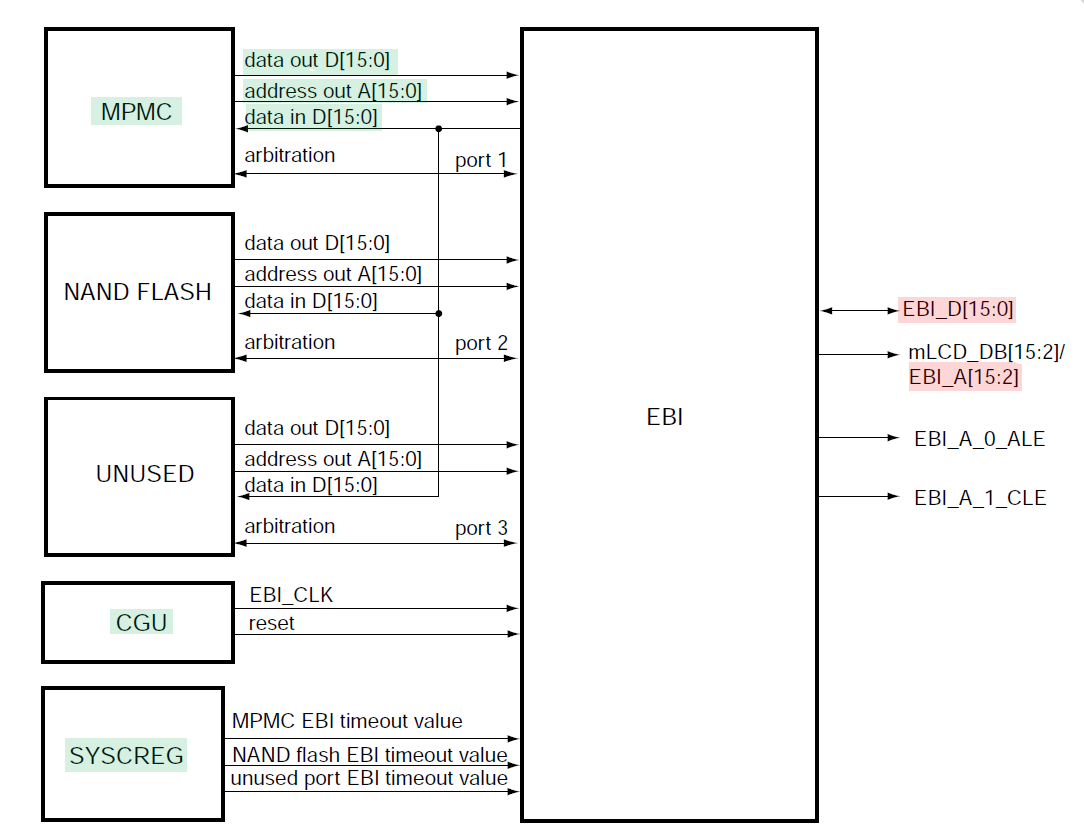
\includegraphics[width=1.0\textwidth]{TeilA/lpc_ebi.png}}
	\caption{NXP LPC313x EBI, Quelle: \cite{NXP2010}}
	\label{fig:lpc_ebi}
\end{figure}
%\end{minipage}

In \refa{fig:lpc_ebi} ist ein Blockschaltbild des EBI zu sehen, bei welchem neben CGU \footnote{CGU: Clock Generation Unit, Takterzeugung} und SYSCREG\footnote{SYSCREG: System Control Register, Steuerregister}, MPMC\footnote{MPMC: Multiport Memory Controller} sowie das NAND Flash an den Eingängen des EBI angeschlossen sind. Abgesehen von NAND Flash sind die Eingänge zum EBI für diese Arbeit relevant und grün markiert. An den Ausgängen des EBI sind Adress- und Datenbus zum Anschluss an externe Bausteine herausgeführt. Damit verschiedenartigen Bausteine an denselben Adress- und Datenpins angeschlossen werden kann, ist eine Priorisierung notwendig. Die Höchste Priorität besitzt der MPMC, gefolgt vom NAND Flash. 
Die Grundidee ist, das Display über den MPMC anzuschließen, da er so konfiguriert werden kann, dass er sich 8080-konform verhält. Die für diese Arbeit interessanten Leitungen am Ausgang des EBI sind mit rot markiert. Hier wird der Datenbus selbst, sowie die oberen 13 Bit des Adressbus gezeigt.


\subsection{MPMC - Multiport Memory Controller des NXP LPC313x}
\label{cha:mpmc}

Der MPMC stellt die Möglichkeit zur Verfügung Bausteine wie dynamisches und statisches RAM anzubinden. Die Refresh-Zyklen werden bei Verwendung von dynamischen RAMs automatisch vollzogen. Das SDRAM-Interface bietet von Haus aus die Möglichkeit Displays mit 8080-Interface zu betreiben. Dies schließt allerdings die Verwendung von dynamischen RAMs aus. Soll ein Betriebssystem wie Linux auf dem System betrieben werden, ist allerdings die Verwendung von dynamischem RAM unerlässlich. Im Folgenden wird die Schnittstelle für das statische RAM SRAM-Interface benannt. Es besteht die Möglichkeit das Interface des statischen RAM zu verwenden, um ein Display zu betreiben, da es sich so konfigurieren lässt, dass es sich wie ein 8080-Interface verhält. Damit sich die verschiedenen Slaves an Adress- und Datenbus nicht überschneiden, regelt das EBI den Zugriff auf die Busse über Chip-Select Leitungen. Am Gnublin ist eine dieser Chip-Select-Leitungen für das SRAM-Interface nach außen gelegt. Die restlichen Anschlüsse wie Write-Enable, Read-Enable, Reset sind ebenfalls herausgeführt \cite{NXP2010}. Ein Blockschaltbild des MPMC ist in \refa{fig:lpc_mpmc} zu sehen.


\begin{figure}[tbph]
%\begin{figure}[h!]
	\centering
\fbox{	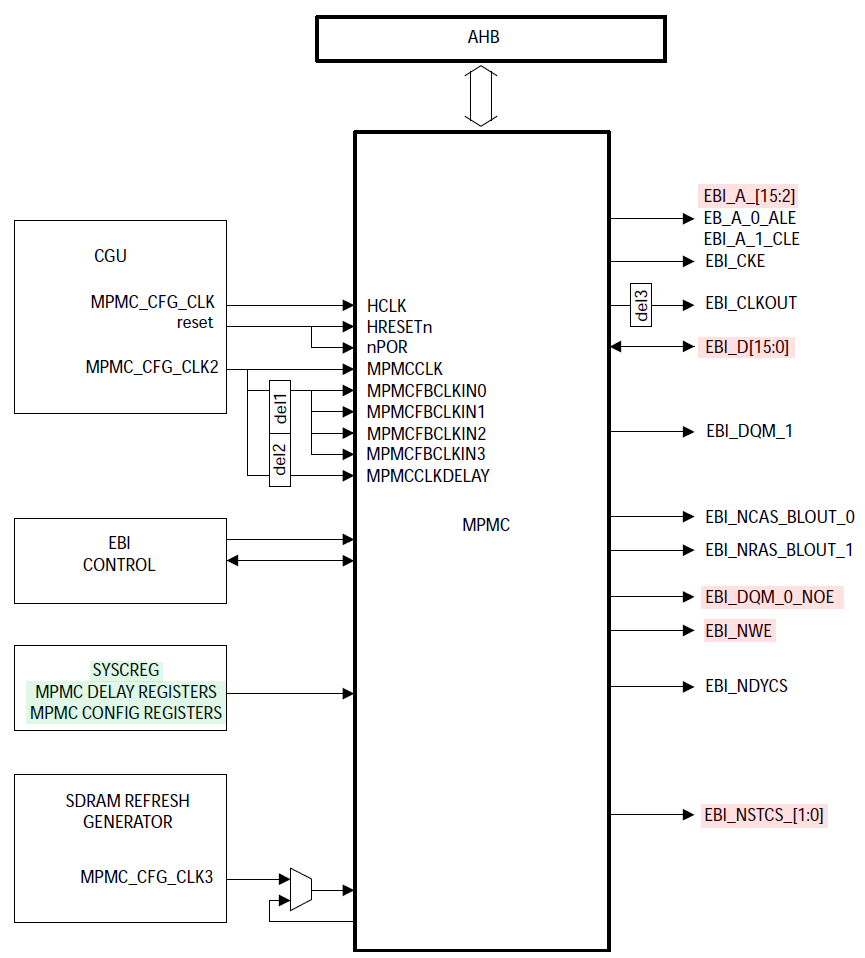
\includegraphics[width=1.0\textwidth]{TeilA/lpc_mpmc.png}}
	\caption{NXP LPC313x MPMC, \cite{NXP2010} }
	\label{fig:lpc_mpmc}
\end{figure}
\newpage
Die Register des MPMC werden so konfiguriert, dass die Schnittstelle kompatibel zum Display und dessen Timings wird. Entsprechend dem verwendeten Chip-Select-Signal werden die Register \begin{itemize}
\item MPMCStaticConfig0
\item  MPMCStaticWaitWen0
\item  MPMCStaticWaitOen0
\item  MPMCStaticRd0
\item  MPMCStaticPage0
\item  MPMCStaticWr0
\item MPMCStaticWaitTurn0 
\end{itemize} konfiguriert. Die Basisadresse des MPMC ist 0x1700 8000. Wie die Register zu beschreiben sind, geht aus \cite{NXP2010} auf Seite 56 hervor und ist in \reft{tab:mpmc_config} gezeigt. Die Timings wurden so gewählt, dass die Timinganforderungen der Displaycontroller eingehalten werden.

\begin{table}[h]
\begin{tabular}{|p{4cm}|p{1cm}|p{1cm}|p{6.6cm}|}\hline
\rowcolor{TableBackgroundColor} 
	\textbf{Register} 	& \textbf{Offset} 	& \textbf{Wert} & \textbf{Beschreibung} 							\\ \hline
	MPMCStaticConfig0 	& 0x200 		& 0x81 			& \begin{itemize}
	\item 16 Bit Modus \item Aktiviert die Nutzung von EBI\_nWE \item  CS low aktiv\item  keine ExtendedWait-Zyklen\item  Schreibpuffer deaktiviert\item  Geschütztes Schreiben deaktiviert \item Page Mode deaktiviert 	\end{itemize} 	\\ \hline
	MPMCStaticWaitWen0 	& 0x204 		& 13 			& 13 + 1 = 14 Wartezyklen ab Chip-Select bis Write-Enable 	\\ \hline
	MPMCStaticWaitOen0 	& 0x208 		& 0 			& 0 + 1 = 1 Wartezyklus ab Chip-Select bis Output-Enable  												\\ \hline
	MPMCStaticRd0 		& 0x20C 		& 0 			& 0 + 1 = 1 Wartezyklus ab Chip-Select bis Read-Enable					\\ \hline
	MPMCStaticPage0 	& 0x210 		& 0 			& 0 + 1 = 1 Wartezyklus für sequential Page Mode Access												\\ \hline
	MPMCStaticWr0 		& 0x214 		& 15 			& 15 + 2  = 17 Wartezyklen bis Write-Access	\\ \hline
	MPMCStaticWaitTurn0 & 0x218 		& 0 			& 0 + 1 = 1 Turnaround Cycles 								\\ \hline
\end{tabular}
\caption{MPMC Register, \cite{NXP2010}}
\label{tab:mpmc_config}
\end{table}
\newpage

Neben den MPMC-Registern muss das Register SYSCREG\_AHB\_MPMC\_MISC konfiguriert werden. Wird Bit 7 des Registers  auf der Adresse 0x1300 2864 mit dem Wert 0 eingestellt, so verändert sich das Adressierungsverhalten dahingehend, dass sich die Adressleitungen des EBI EBI\_A[15:0] auf den für den Prozessor sichtbaren AHB\footnote{AHB: Advanced Microcontroller Bus Architecture} Adressbus AHB\_A[16:1] verschiebt (siehe \cite{NXP2010}, S.~485f). Der Prozessor selbst, kann nun also 17 Bit adressieren, jedoch nur im Sprung von zwei Adressen, da das ursprüngliche LSB weggefallen ist.

\newpage
\subsection{Hardwareverbindung zwischen SRAM-Interface und Display}
In diesem Abschnitt wird die Verbindung zwischen dem Prozessor und dem Display behandelt. Eingangs wurde bereits erwähnt, dass beim Kauf der Displays Augenmerk auf Pinkompatibilität gelegt wurde. Das schlägt sich beim Entwurf der Adapterplatine positiv zu Buche, da nun lediglich ein Adapter benötigt wird. \newline
Bereits dargestellt zeigt \refa{fig:8080_pinout} auf Seite \pageref{fig:8080_pinout} das Pinout der verwendeten Displays. Der Anschluss an den Prozessor stellt sich wir in \reft{tab:display_gnublin_verbindung} dar. Anhand der gewonnenen Erkenntnisse aus \refc{cha:teila_konzept} und \refc{cha:mpmc} sowie des Schaltplans des verwendeten Gnublin Extended (siehe \cite{EmbeddedProjects2013}) kann eine Zuordnung getroffen werden. Nicht verbundene Pins sind mit 'nc'\footnote{nc: not connected} vermerkt.

\begin{table}[h]
\begin{tabular}{|p{0.6cm}|p{2.5cm}|p{2.5cm}|p{0.6cm}|p{2.5cm}|p{2.5cm}|}\hline
\rowcolor{TableBackgroundColor} 
\textbf{Nr.}	&	\textbf{Pin Display}	&	\textbf{Pin Gnublin}  & \textbf{Nr.}	&	\textbf{Pin Display}	&	\textbf{Pin Gnublin} 	\\ \hline
1				&	GND						&	GND					  &	21				&	DB0						&	LPC\_DB0				\\ \hline
2				&	+3V3					&	+3V3				  &	22				&	DB1						&	LPC\_DB1				\\ \hline
3				&	nc						&	nc				 	  & 23				&	DB2						&	LPC\_DB2				\\ \hline
4				&	RS						&	LPC\_A15	    	  &	24				&	DB3						&	LPC\_DB3				\\ \hline
5				&	WR						&	LPC\_WE				  &	25				&	DB4						&	LPC\_DB4				\\ \hline
6				&	RD						&	LPC\_DQM0			  &	26				&	DB5						&	LPC\_DB5				\\ \hline
7				&	DB8						&	LPC\_DB8			  &	27				&	DB6						&	LPC\_DB6				\\ \hline
8				&	DB9						&	LPC\_DB9			  &	28				&	DB7						&	LPC\_DB7				\\ \hline
9				&	DB10					&	LPC\_DB10			  &	29				&	nc						&	nc						\\ \hline
10				&	DB11					&	LPC\_DB11			  &	30				&	nc						&	nc						\\ \hline
11				&	DB12					&	LPC\_DB12			  &	31				&	nc						&	nc						\\ \hline
12				&	DB13					&	LPC\_DB13			  &	32				&	nc						&	nc						\\ \hline
13				&	DB14					&	LPC\_DB14			  &	33				&	nc						&	nc						\\ \hline
14				&	DB15					&	LPC\_DB15			  &	34				&	nc						&	nc						\\ \hline
15				&	CS						&	STCS0				  &	35				&	nc						&	nc						\\ \hline
16				&	nc						&	nc					  &	36				&	nc						&	nc						\\ \hline
17				&	RESET					&	GPIO19				  &	37				&	nc						&	nc						\\ \hline
18				&	nc						&	nc					  &	38				&	nc						&	nc						\\ \hline
19				&	LED-A					&	GPIO20				  &	39				&	nc						&	nc						\\ \hline
20				&	nc						&	nc				 	  &	40				&	nc						&	nc						\\ \hline

\end{tabular}
\caption{Displayverbindung mit dem Gnublin, \cite{Coldtears2014}, \cite{EmbeddedProjects2013}}
\label{tab:display_gnublin_verbindung}
\end{table}

Das Daten-Interface des Displays ist mit den Pins DB[0:15] mit dem Datenbus verbunden. Die Signale Read-Enable RD und Write-Enable WR liegen auf den Pins LPC\_DQM0 und LPC\_WE. Als Chip-Select wird das Signal STCS0 verwendet. Diese Pins sind aus dem EBI herausgeführt (siehe \refa{fig:lpc_ebi}) und werden, sofern es das System von der Auslastung am Bus ermöglicht, für das Display zur Verfügung gestellt.

Das RS Signal am Display, welches zwischen Kommando und Daten unterscheidet, liegt auf dem Adresssignal A15. Die folgenden Angaben gehen von einer Registerkonfiguration nach \refc{cha:mpmc} aus. Werden Daten gesendet, so ist der Pin logisch 1, was einem Wert auf dem Adressbus von 0x10000\footnote{0x10000 = 0b0001 0000 0000 0000 0000} entspricht. Bei Kommandos ist der Pin logisch 0 mit einem Adresswert von 0x00000\footnote{0x00000 = 0b0000 0000 0000 0000 0000}. Die unteren 16 Bits des Adressraums lassen sich also willkürlich verändern, da nur das MSB\footnote{MSB: Most Sigificant Bit, das höchstwertige Bit} vom Display verwendet wird. 

Als RS-Pin ist die Adressleitung A15 (logisch verschoben auf A16) gewählt, da so möglicherweise DMA-Transfers\footnote{DMA: Direct Memory Access, Speichertransfer effizient und schnell direkt in Hardware} von bis zu 65.536 Bytes\footnote{65.536 = $2^{16}$} möglich sind. Der DMA-Transfer könnte die Adressleitungen bei Daten von 0x10000 bis 0x1FFFF\footnote{0x1FFFF = 0b0001 1111 1111 1111 1111} bzw. bei Kommandos von 0x0000 bis 0x0FFFF\footnote{0x0FFFF = 0b0000 1111 1111 1111 1111} inkrementieren ohne die Gültigkeit der Wahl zwischen Kommando und Daten des Displays zu beeinträchtigen.

Das Display lässt sich Zusammenfassend also über zwei Pseudoregister für Kommando und Daten auf den Adressoffsets 0x00000 und 0x10000 mit der Basisadresse 0x20000000 ansprechen. Dies ist in \reft{tab:sram_adressen} nochmals übersichtlich dargestellt.

\begin{table}[h]
\begin{tabular}{|p{4.5cm}|p{4cm}|p{4cm}|}\hline
\rowcolor{TableBackgroundColor} 
	\textbf{Register} 	& \textbf{Adresse} 	& \textbf{Typ} 			\\ \hline
	SRAM0\_DISP\_CTRL 	& 0x20000000		& Kommandos				\\ \hline
	SRAM0\_DISP\_DATA 	& 0x20010000 		& Daten 				\\ \hline
\end{tabular}
\caption{Adressen für SRAM-Zugriff, \cite{NXP2010}}
\label{tab:sram_adressen}
\end{table}


Die Untersuchung inwieweit DMA-Transfer praktisch mit der verwendeten Hardware möglich ist, ist allerdings nicht Bestandteil dieser Arbeit. 

\newpage
\subsection{Adapterplatine zwischen Gnublin Extended und Display}
Der Adapter wird als Platine realisiert, die auf den Gnublin Extended aufgesteckt wird. Das Display wiederum wird mit der Adapterplatine steckbar verbunden. Der Schaltplan ist in \refa{fig:adapterplatine_sch} gezeigt und stellt entsprechend \reft{tab:display_gnublin_verbindung} die Verbindungen her.

Der grün markierte Bereich stellt die Verbindung zum Display dar, rot zum Gnublin Extended und im blauen Rechteck sind weitere kleine Bauteile untergebracht. Hier sind Pullup-Wiederstande mit 10~k$\Omega$ an den Leitungen STCS0, Reset und LED-A um definierte Pegel vorzugeben zu sehen sowie einen Blockkondensator mit 100~nF, der für eine bessere Spannungsversorgung des Displays sorgt.

\begin{figure}[tbph]
%\begin{figure}[h!]
	\centering
\fbox{	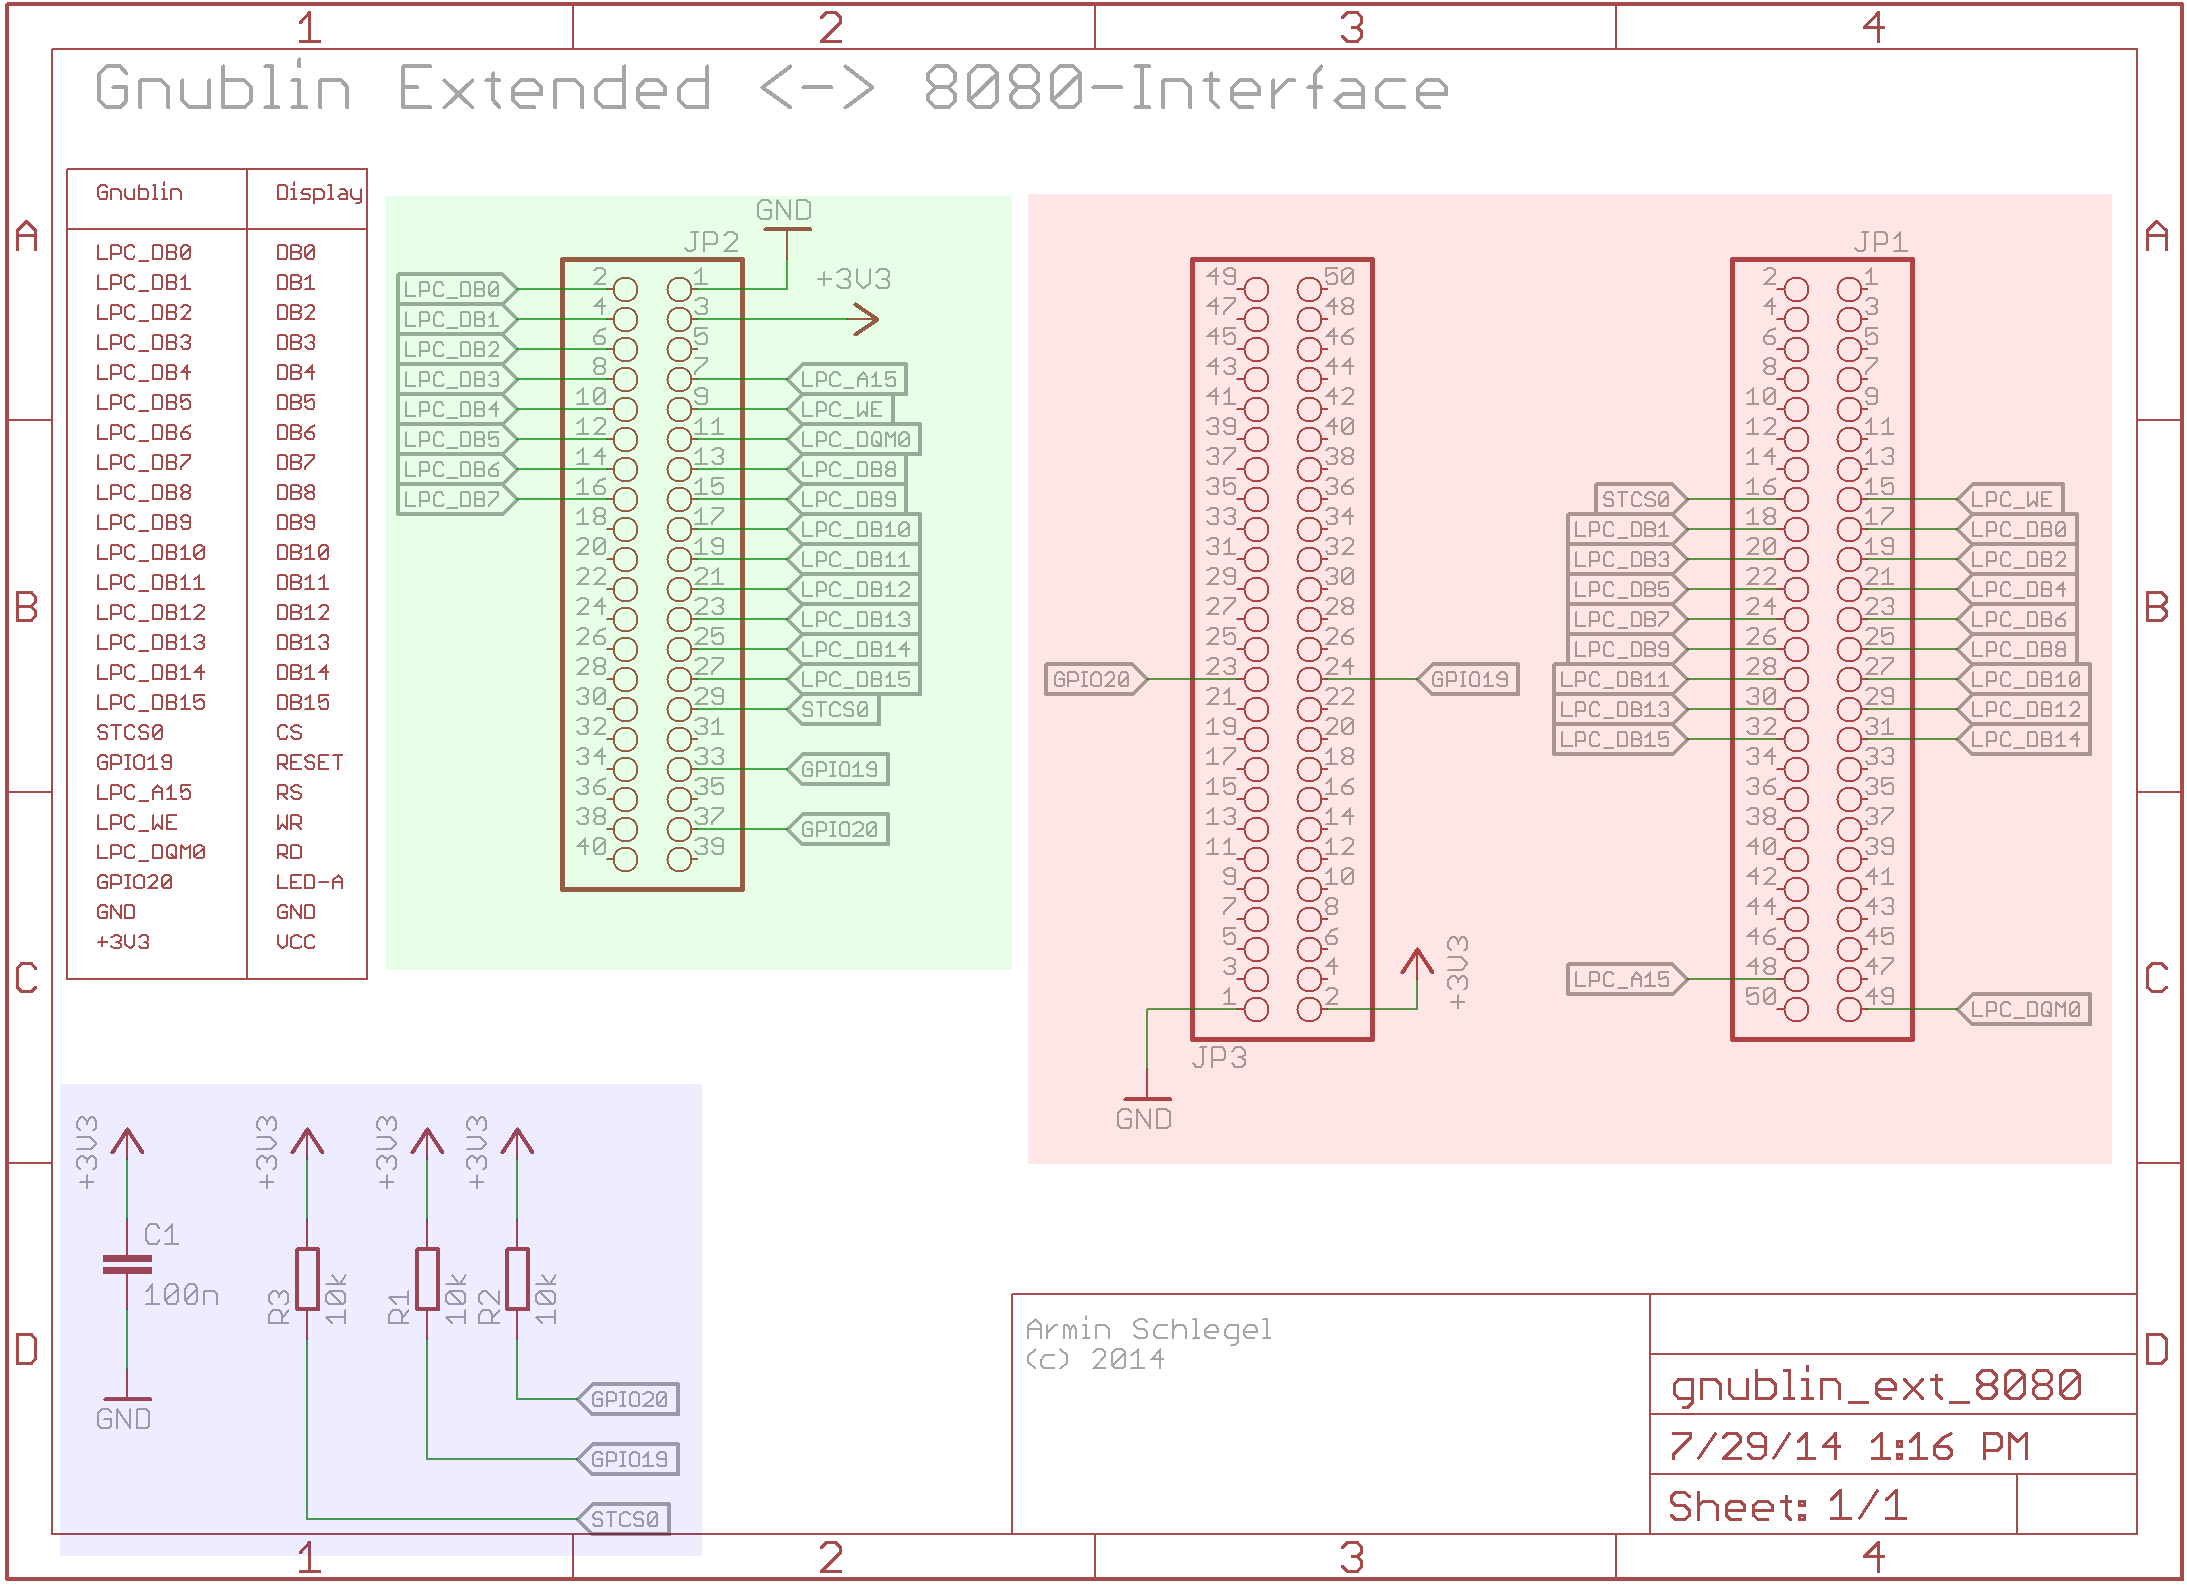
\includegraphics[width=1.0\textwidth]{TeilA/schematic.png}}
	\caption{Schaltplan Adapterplatine}
	\label{fig:adapterplatine_sch}
\end{figure}
\newpage

\refa{fig:adapterplatine} (a) und (b) zeigt je ein gerendertes 3D Bild der Ober- und Unterseite der Adapterplatine. Auf der Oberseite wird das Display auf der linken Seite mit der 40 poligen Stiftleiste angeschossen. Mit der Unterseite wird die Platine auf das Gnublin Extended mit je zwei 50 poligen Buchsenleisten aufgesteckt.

\begin{figure}
        \begin{center}
        \begin{subfigure}[htp]{0.8\textwidth}
                \fbox{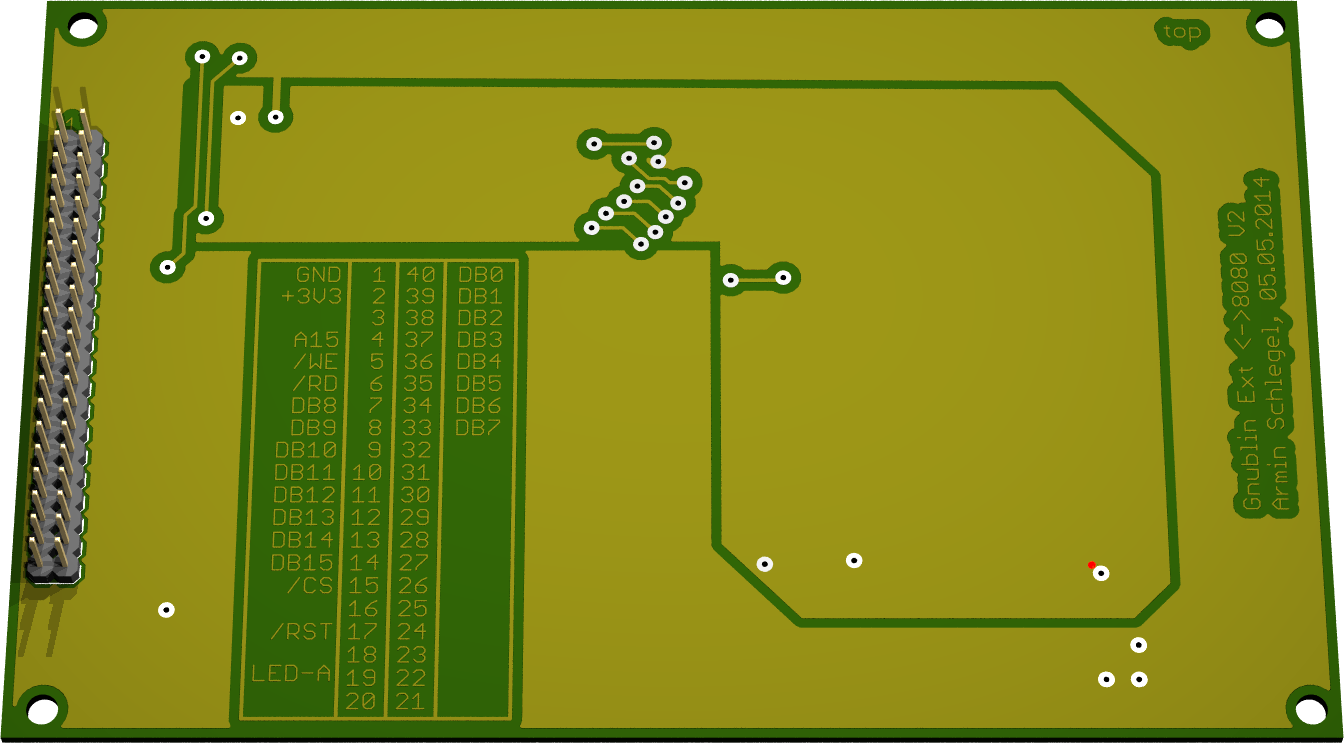
\includegraphics[width=\textwidth]{TeilA/gnublin_ext_ssd1963_top.png}}
                \caption{Adapterplatine Top Layer}
                \label{fig:adapter_top}
        \end{subfigure}

        \begin{subfigure}[htp]{0.8\textwidth}
               \fbox{ 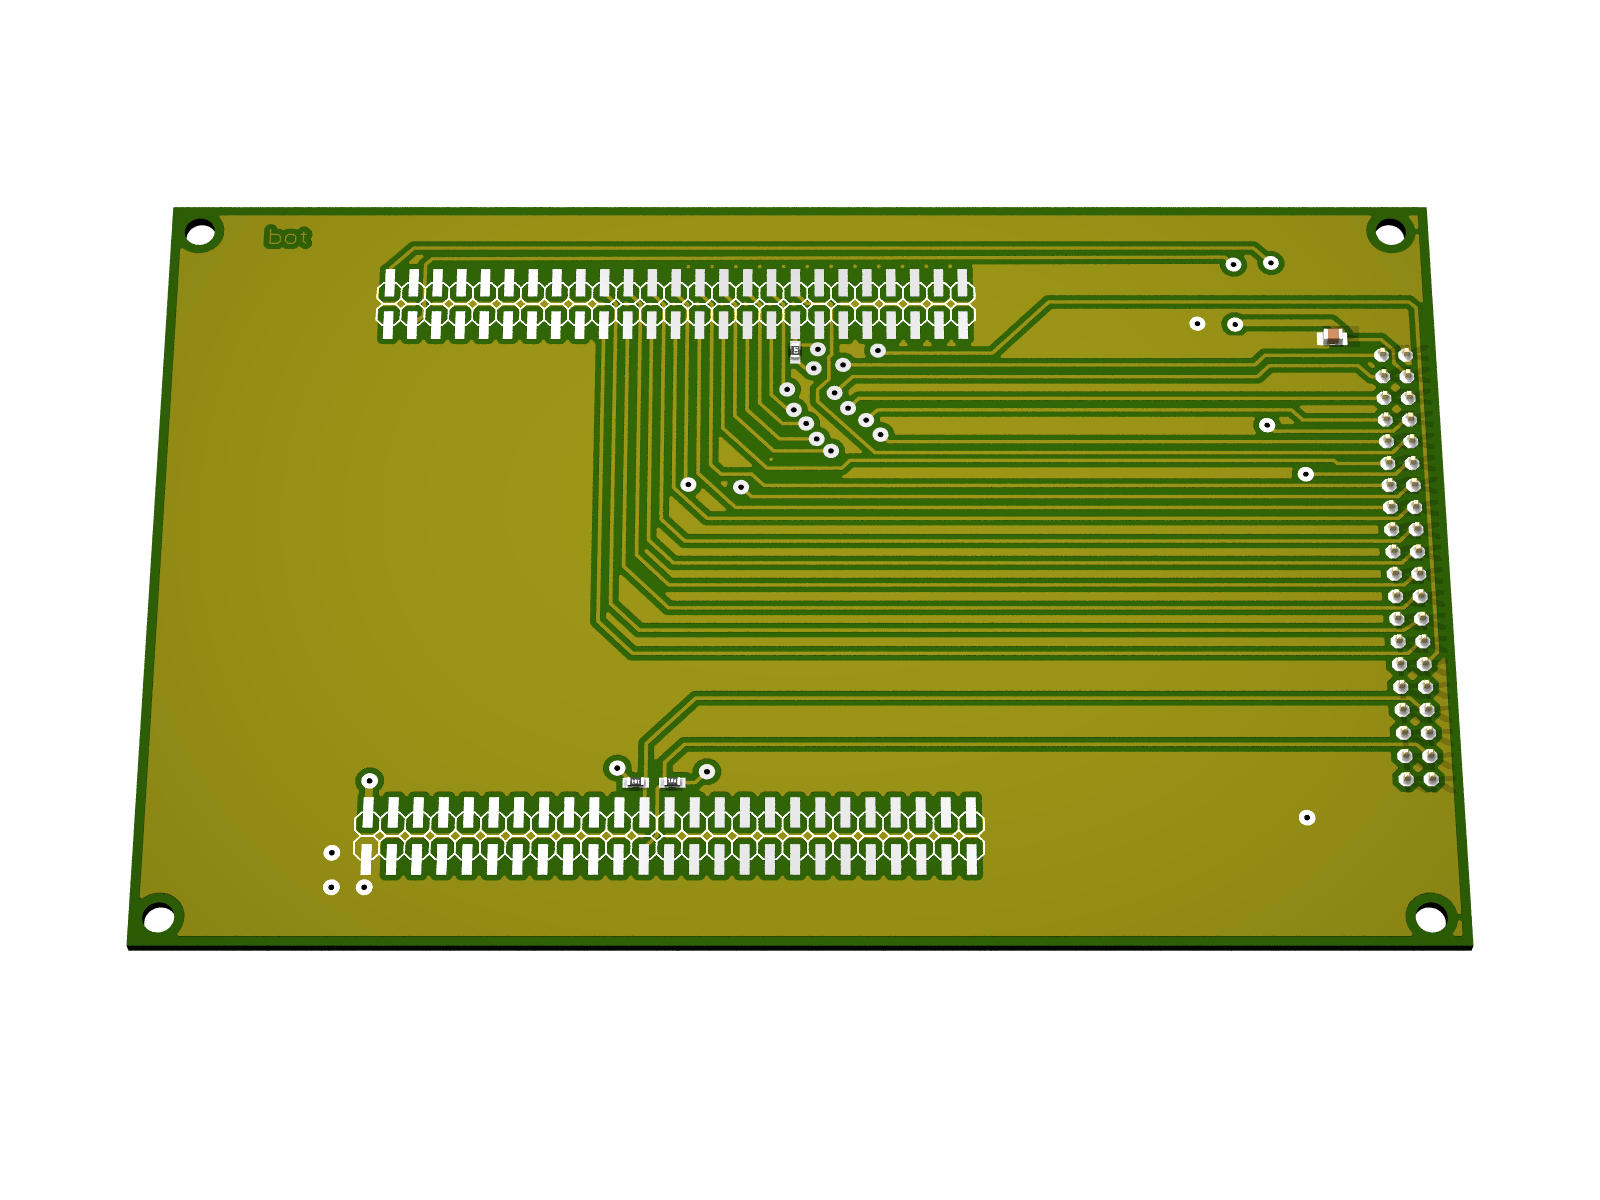
\includegraphics[width=\textwidth]{TeilA/gnublin_ext_ssd1963_bot.png} }              				\caption{Adapterplatine Bottom Layer}
                \label{fig:adapter_bot}
        \end{subfigure}
		\end{center}
        \caption{Adapterplatine zwischen Gnublin Extended und Display}\label{fig:adapterplatine}
\end{figure}

Die Schaltplan und das Layout befinden sich in der CD im Anhang dieser Arbeit.
\newpage
\subsection{Software}
Im Folgenden Abschnitt wird die Software behandelt, die nötig ist, um das Display zu betreiben. 
Die Softwareentwicklung ist in drei Teile auf gegliedert:
\begin{itemize}
\item Modifikationen im Bootloader APEX
\item Framebuffer-Treiber im Linux-Kernel
\item Userspace-Treiber basierend auf einem Treibers auf für den Raspberry Pi (siehe \cite{Schlegel2013a} und \cite{Schlegel2013b}) bei dem mittels GPIO-Pins ein 8080-Display zu betreiben
\end{itemize}

\subsubsection{Anpassung des APEX-Bootloaders zur Verwendung des Displays}
Der APEX-Bootloader\footnote{\url{https://gitorious.org/apex/}} wurde ursprünglich für Prozessoren de Sharp LH Familie entwickelt, wurde allerdings auf eine Vielzahl von weiteren ARM basierten Prozessoren portiert, so auch für die verwendete NXP LPC313x CPU\footnote{CPU: Central Processing Unit, Prozessor}.
Die Aufgabe des Bootloaders ist es, grundlegende prozessorinterne Hardwareeinheiten wie z.B. CGU oder SD-RAM zu initialisieren um für den Linux-Kernel die notwendige Umgebung zu schaffen. Im Anschluss wird der Linux-Kernel geladen und gestartet. Es werden außerdem dem Linux-Kernel Bootparameter übergeben, die zum Start benötigt werden. Am Anfang des Bootloader-Codes werden die verwendeten MPMC-Register konfiguriert. Wie in \refc{cha:mpmc} muss das SYSCREG-Register SYSCREG\_AHB\_MPMC\_MISC nicht explizit beschrieben werden, da es im Resetzustand bereits richtig konfiguriert ist. \refl{lst:apex_mpmc_config} zeigt die entsprechende Initialisierung der MPMC-Register für das MD050SD. Die Adressen von z.B. MPMC\_STCONFIG0 sind in der \code{lpc313x.h} definiert. Die Modifikationen im Bootloader finden in der Datei \code{initialize.c} statt.

\begin{lstlisting}[%
language=MyC,
caption={Bootloader: MPMC-Konfiguration},
label=lst:apex_mpmc_config
]
#elif defined(CONFIG_MACH_EPLPC3131_V1)
#if defined(CONFIG_DISP_SSD1963)
	// ...
#elif defined(CONFIG_DISP_MD050SD)
   /* LCD display, 16 bit */
   MPMC_STCONFIG0  = 0x81;
   MPMC_STWTWEN0   = 13;
   MPMC_STWTOEN0   = 0;
   MPMC_STWTRD0    = 0;
   MPMC_STWTPG0    = 0;
   MPMC_STWTWR0    = 15;
   MPMC_STWTTURN0  = 0;
#elif defined(CONFIG_DISP_SSD1289)
	// ...
#elif defined(CONFIG_DISP_NONE)
	// ...
#endif
#endif
\end{lstlisting}


\paragraph{Boot-Logo im APEX-Bootloader}
\label{cha:bootloader}
Um dem Display beim Systemstart einen initialisierten Zustand zu geben und dem Benutzer bereits während dem Laden des Linux-Kernels ein Bild anzuzeigen, ist ein Bootlogo konfigurierbar. Hierfür bedarf es eines rudimentären Displaytreibers im Bootloader. Im Folgenden wird die Darstellung des Boot-Logos unter Verwendung des MD050SD dargestellt. \refl{lst:apex_erster_teil} zeigt den ersten Teil des Treibers, bei dem grundlegende Datentypen sowie Sendefunktionen für Daten und Kommandos gelistet sind. 

\begin{lstlisting}[%
language=MyC,
caption={Bootloader: Grundlegende Datentypen und Funktionen},
label=lst:apex_erster_teil
]
#if defined(CONFIG_DISP_MD050SD) || defined(CONFIG_DISP_SSD1963) || defined(CONFIG_DISP_SSD1289)
#define DISP_PHYS        (EXT_SRAM0_PHYS)
#define DISP_PHYS_CTRL   (DISP_PHYS + 0)
#define DISP_PHYS_DATA   (DISP_PHYS + 0x10000)

unsigned int width;
unsigned int height;
int pixel;

struct display {
   volatile u16* ctrl;
   volatile u16* data;
};

static struct display display;

static void display_send_cmd(u16 cmd)
{
   *display.ctrl = 0x00FF & cmd;
}

static void display_send_data(u16 data)
{
   *display.data = data;
}

#endif
\end{lstlisting}

Die Struktur \code{struct display} ab Zeile 10 von \refl{lst:apex_erster_teil} enthält zwei Zeiger \code{u16* ctrl} und \code{u16* data} auf die jeweiligen Adressen aus \reft{tab:sram_adressen} für Kommandos und Daten. In den Zeilen 17 und 22 sind die zwei Sendefunktionen \code{display\_send\_cmd(u16 cmd)} und 
\code{display\_send\_data(u16 cmd)} definiert. Hiermit werden die Kommandos und Daten an das Display gesendet. Wird auf eine der beiden Adressen ein Wert geschrieben, kümmert sich das MPMC und das EBI automatisch um die restlichen Signale wie WR, RD und CS. 

\begin{lstlisting}[%
language=MyC,
caption={Bootloader: Display-Initialisierung und Bootlogo},
label=lst:apex_zweiter_teil
]
#if defined(CONFIG_DISP_MD050SD) || defined(CONFIG_DISP_SSD1963) || defined(CONFIG_DISP_SSD1289)
   display.ctrl = &__REG16 (DISP_PHYS_CTRL);   
   display.data = &__REG16 (DISP_PHYS_DATA); 
#if defined(CONFIG_DISP_MD050SD)
   GPIO_OUT_LOW(IOCONF_GPIO, _BIT(14)); //GPIO20 is LED_ENABLE

   GPIO_OUT_LOW(IOCONF_GPIO, _BIT(13)); //GPIO19 is nRESET
   udelay(20000);
   GPIO_OUT_HIGH(IOCONF_GPIO, _BIT(13)); //GPIO19 is nRESET
   udelay(20000);

	/* Set Window from 0,0 to 479, 799 */
   display_send_cmd(0x0002);			
   display_send_data(0);				
   display_send_cmd(0x0003);			
   display_send_data(0);				

   display_send_cmd(0x0006);
   display_send_data(480 - 1);
   display_send_cmd(0x0007);
   display_send_data(800 - 1);

	/* Clear the display with color black */
   display_send_cmd(0x000F);

   for(pixel = 0; pixel < 800 * 480; pixel++)
   {
      display_send_data(0x0000);
   }

   GPIO_OUT_HIGH(IOCONF_GPIO, _BIT(14)); //GPIO20 is LED_ENABLE

#if defined(CONFIG_LOGO_TUX)
   width = boot_logo_tux[0];
   height = boot_logo_tux[1];

   display_send_cmd(0x0002);
   display_send_data(480/2 - (height - 1)/2);
   display_send_cmd(0x0003);
   display_send_data(800/2 - (width - 1)/2);
   display_send_cmd(0x0006);
   display_send_data(480/2 + (height - 1)/2 + 1);
   display_send_cmd(0x0007);
   display_send_data(800/2 + (width - 1)/2 + 1);
   display_send_cmd(0x000F);

   for(pixel = 2; pixel < width * height + 2; pixel++)
   {
      display_send_data(boot_logo_tux[pixel]);
   }
#endif
#endif
#endif
\end{lstlisting}

Der Eigentliche Treiber und der Code für das Anzeigen des Bootlogos ist in \refl{lst:apex_zweiter_teil} zu sehen. In Zeile 2 und 3 werden den Adresszeigern die pysikalischen Adressen zum Schreiben von Kommandos und Daten zugewiesen. Von Zeile 5 bis 10 wird die Hintergrundbeleuchtung explizit abgschaltet und ein Reset auf das Display gegeben. Da das MD050SD einen CPLD-Controller besitzt, welcher eine auf genau dieses TFT-Panel zugeschnittene Programmierung enthält, fällt eine Initialisierungsroutine weg. Dies wäre bei Controllern wie dem SSD1963 nicht der Fall, da diese mit einer Vielzahl von Panels arbeiten können und demzufolge eine spezielle Initialisierung brauchen. Das MD050SD ist nach dem Reset also initialisiert und erwartet Kommandos. Von Zeile 13 bis 24 in \refl{lst:apex_zweiter_teil} wird ein Bereich im Display-RAM der vollen Bildschirmgröße reserviert und die Bereitschaft zum Datenempfang gestartet (siehe \reft{tab:Kommandos_MD050SD}). Alle Daten die im Anschluss gesendet werden, werden automatisch an die richtige Stelle im Display geschrieben. In einer Schleife werden ab Zeile 26 alle reservierten Pixel von zuvor mit der Farbe Schwarz beschrieben, um das automatisch angezeigte Testbild des Displays beim Start zu überschreiben. Im Anschluss wird die Hintergrundbeleuchtung wieder eingeschaltet. Ist über den Codeswitch \code{CONFIG\_LOGO\_TUX} das Bootlogo aktiviert, so wird dies ab Zeile 34 angezeigt. Die Größe des Logos wird in den Zeilen 34 und 35 ausgelesen und in den Folgenden angezeigt. Die Pixeldaten des Logos sind im Array \code{u16 boot\_logo\_tux[]} in den Dateien \code{boot\_logo\_tux.c} und \code{boot\_logo\_tux.h} hinterlegt.


\paragraph{Konfiguration des APEX-Bootloaders}
\label{cha:config_apex}
Der APEX-Bootloader besitzt zur Konfiguration dasselbe System wie der Linux-Kernel. Dieses System heißt KConfig und wird durch den Befehl \code{make menuconfig} aufgerufen, welches ein Konfigurationsmenü im aufrufenden Terminal erscheinen lässt. Hier sind neben Grundlegenden Konfiguration zum Beispiel für die Prozessorarchitektur oder Taktraten auch der Displaytreiber und das Bootlogo eingepflegt. \refa{fig:apex_config} zeigt exemplarisch den Unterpunkt \code{Platform Setup} bei dem das Display MD050SD und das Bootlogo ausgewählt sind. 

\begin{figure}[tbph]
%\begin{figure}[h!]
	\centering
\fbox{	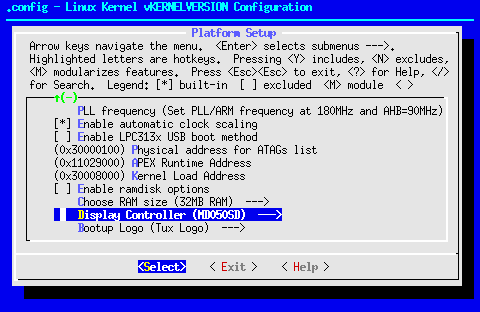
\includegraphics[width=0.8\textwidth]{TeilA/apex_config.png}}
	\caption{APEX-Bootloader KConfig}
	\label{fig:apex_config}
\end{figure}
\newpage

Bevor der Bootloader konfiguriert werden kann, muss der Vanilla-Quellcode\footnote{Vanilla-Quellcode: unmodifizierter, originaler Quellcode} noch gepatcht werden. \refl{lst:apex_patchen} zeigt die einzelnen Schritte, um den Bootloader herunterzuladen und zu Patchen. Der Patch enthält alle nötigen Dinge zum Betrieb des MD050SD-Display und des Boot-Logos.

\begin{lstlisting}[%
language=bash,
caption={Bootloader: Bootloader herunterladen und patchen},
label=lst:apex_patchen
]
$ wget https://github.com/embeddedprojects/gnublin-distribution/raw/master/lpc3131/bootloader/apex/1.6.8/apex-1.6.8.tar.gz
$ tar xvfz apex-1.6.8.tar.gz
$ wget https://github.com/siredmar/master/raw/master/Teil_A/software/bootloader/apex_display.patch
$ cd apex-1.6.8
$ patch -p1 < ../apex_display.patch
\end{lstlisting}

Im Folgenden wird die Konfiguration des Bootloaders und die damit möglichen Einstellungsmöglichkeiten beschrieben. Im Konfigurationsmenü sind nach dem patchen im Untermenü \code{Platform Setup} die Optionen \code{Display Controller} und \code{Bootup Logo} verfügbar. Hier wird die Auswahl bezüglich Displaycontrollers und Logo getroffen. Wird ein Displaycontroller anders als MD050SD gewählt, so werden nur entsprechende Timings der MPMC-Register gesetzt und kein Boot-Logo angezeigt. 
Um den Kernel mit spezifischen Parametern starten zu können, werden für den Betrieb der unterschiedlichen Treiber (Framebuffer, User-Space) andere Bootparameter benötigt. So ist der originalen Parameterliste \code{console=ttyS0,115200n8 root=/dev/mmcblk0p3 rw rootfstype=ext4 rootwait} im Untermenü \code{Environment} für den Betrieb mit dem Framebuffer-Treiber ein \code{fbcon=rotate:0 fbcon=font:VGA8x16} hinzuzufügen um dem Kernel beim Start Informationen über den Kernel-Treiber \code{fbcon} mitzuteilen. Wird der User-Space-Treiber verwendet, so übernimmt das Kernel-Modul \code{vfb}\footnote{vfb: Virtual Frame Buffer} die Aufgabe des Framebuffers. Die Parameterliste ist mit \code{console=tty0 video=vfb: vfb\_enable=1} zu ergänzen (siehe \cite{LinuxKernelFBCON}).

Der Bootloader wird per \code{make apex.bin} kompiliert und mit \code{dd if=src/arch-arm/rom/apex.bin of=/dev/sdXY} \footnote{/dev/sdXY: bezieht sich auf die Bootpartition auf der korrekten SD-Karte, z.b. /dev/sdb2} auf die SD-Karte des Gnublin geschrieben (siehe \cite{GnublinWiki2013a}).

\subsubsection{Entwicklung eines Linux-Framebuffer-Treibers}
Für den Betrieb des Gnublin Extended wird die offizielle Version des Kernels aus dem Git-Repository von Embedded Projects für die Architektur NXP LPC313x in der Kernelversion 2.6.33 verwendet (siehe \cite{GnublinWiki2013b}). Um mit den Displays zusammenzuarbeiten, muss dieser mit dem entwickelten Treiber gepatcht werden. \refl{lst:kernel_patchen} zeigt die einzelnen Schritte, die dafür notwendig sind.

\begin{lstlisting}[%
language=bash,
caption={Framebuffer: Kernel herunterladen und patchen},
label=lst:kernel_patchen
]
$ git clone https://github.com/embeddedprojects/gnublin-lpc3131-2.6.33.git
$ cd gnublin-lpc3131-2.6.33
$ wget https://github.com/siredmar/master/raw/master/Teil_A/software/linux/display_drivers.patch
$ cd linux-2.6.33-lpc313x
$ make gnublin_defconfig
$ patch -p1 < ../display_drivers.patch
\end{lstlisting}
Wie der Cross-Compiler für die Verwendung der LPC3131x-Architektur installiert wird ist \cite{GnublinWiki2013c} zu entnehmen.

In diesem Abschnitt wird die Entwicklung des Framebuffer-Treibers beschrieben. Der Framebuffer-System bietet eine Abstraktionsebene für die Grafikhardware. Es enthält einen Bildspeicher der Grafikhardware und bietet Applikationen Zugriff auf diesen, ohne jedoch Informationen über die letztendlich verwendete Hardware selbst auf Low-Level-Ebene haben zu müssen. Ein Framebuffer-Device erzeugt die Node \code{/dev/fbX} mit der fortlaufenden Nummer X, beginnend bei Null, für jede Instanz eines Framebuffers. Jede grafische Anwendung in einem Linux-System benötigt eine Funktionalität, die den aktuellen Bildschirminhalt speichert und  Applikationen zugriff darauf gewährt. Dabei ist es im wesentlichen unwichtig, ob die Anzeige selbst durch Hardware beschleunigt oder sogar nur rein virtuell realisiert wird, da die Applikation auf die Schnittstelle in \code{/dev/fbX} zugreift (siehe  \cite{LinuxKernelFB}).
Programme wie zum Beispiel der X11-Server, Video-Player, QT\footnote{QT: C++-Klassenbibliothek zur 2D-Darstellung, \url{http://qt-project.org/}}, SDL\footnote{SDL: Simple Direct Media Layer, Grafikbibliothek zur 2D-Darstellung, \url{http://www.libsdl.org}} usw. können dieses System nutzen. Gerade für leistungsschwächere Systeme bietet es dahingehend dieselben Möglichkeiten Programme Anzuzeigen, wie für High-End-Systeme. Einzig die Art und Weise des Befüllens und Auslesens des Framebuffers unterscheidet die Leistungsfähigkeit einzelner Systeme. So können Systeme mit zusätzlichen Grafikeinheiten die speziell zum Berechnen von 3D-Daten mit zum Beispiel der 3D-Grafikbibliothek OpenGL\footnote{OpenGL: 3D Grafikbibliothek} den Framebuffer mit "'hochwertigeren"' Inhalten füllen, als ein System, das diese Möglichkeit nicht besitzt. Die Abstraktionsebene für die Applikation bleiben aber dieselben. 

Mit der Entwicklung eines Framebuffer-Treibers, sind alle Vorteile erschlossen, welche das Framebuffer-System bietet. Diese sind eine standardisierte Schnittstelle für Applikationen, sowie die Gewissheit, dass, sofern es die Rechenleistung zulässt, prinzipiell alle bereits existenten Programme und Inhalte angezeigt werden können.
In den folgenden Abschnitten, wird die Entwicklung des Framebuffer-Treibers für die drei verwendeten Displays dargelegt, mit Fokus auf das MD050SD. 
\paragraph{Framebuffer-Treiber für MD050SD}
\label{cha:framebuffer}
In diesem Abschnitt wird die Funktionsweise des Framebuffer-Treibers für das MD050SD beschrieben. Auf ein Listing des kompletten Treibers wird an dieser Stelle bewusst verzichtet, da sonst der Treiber durch seine Komplexität und die ins System verflochtene Struktur schwer zu durchdringen wäre. Stattdessen werden einzelne Teilaspekte, die zum Verständnis nötig sind, einzeln behandelt. Als Basis wurde ein bereits existierender Treiber verwendet (siehe \cite{Schlegel2013c}).

Der Treiber arbeitet konform mit dem "'Platform Device"'- und "'Platform Driver"'-System im Linux-Kernel (siehe \cite{LinuxKernelPlatformDeviceDriver}). Mit dem Platform-Device-System wird ein Pseudo-Bus erzeugt, mit dem sich verschiedene Platform-Driver verbinden können. So können beispielsweise mehrere voneinander unabhängige Instanzen eines Treibers oder vieler verschiedener Treiber im System verfügbar sein. Beinhaltet ein System ein Platform-Device, so muss es dem Linux-Kernel bekannt gemacht werden. Hierzu wird die Struktur \code{struct platform\_device} verwendet, die in \refl{lst:struct_platform_device} gezeigt ist.

\begin{lstlisting}[%
language=MyC,
caption={Framebuffer: struct platform\_device},
label=lst:struct_platform_device
]
struct platform_device {
	const char	*name;
	u32		id;
	struct device	dev;
	u32		num_resources;
	struct resource	*resource;
};
\end{lstlisting}

In der Struktur in \refl{lst:struct_platform_device} sind Datentypen enthalten, die einen eindeutigen Namen des Devices \code{const char *name}, sowie eine ID \code{u32 id}  bestimmen, einen Parameter zur Struktur \code{struct device}, sowie einen Zeiger zur Struktur \code{struct resource}, die letztendlich die Hardware-Ressourcen darstellen. Für den Platform-Driver ist die Struktur \code{struct platform\_driver} in \refl{lst:struct_platform_driver} gegeben, die Funktionszeiger für den Betrieb des Treibers und eine Struktur \code{struct device\_driver} enthält, welche zur Zuordnung mit dem entsprechenden Platform-Device dient.
\begin{lstlisting}[%
language=MyC,
caption={Framebuffer: struct platform\_driver},
label=lst:struct_platform_driver
]
struct platform_driver {
	int (*probe)(struct platform_device *);
	int (*remove)(struct platform_device *);
	void (*shutdown)(struct platform_device *);
	int (*suspend)(struct platform_device *, pm_message_t state);
	int (*suspend_late)(struct platform_device *, pm_message_t state);
	int (*resume_early)(struct platform_device *);
	int (*resume)(struct platform_device *);
	struct device_driver driver;
};
\end{lstlisting}

Wie ein Platform-Device definiert wird, ist \refl{lst:register_platform_devices} zu entnehmen. Die Modifikationen sind im Quellcode der Start-Datei der Architektur \code{linux-2.6.33-lpc313x/arch/arm/mach-lpc313x/ea313x.c} eingepflegt. In den Zeilen 2 bis 13 wird die Ressource \code{struct resource md050sd\_resource[]} definiert, die zwei Einträge enthält. Hier werden die physikalischen Adressen für Kommandos und Daten  für das Display auf SRAM-Interface eingestellt, die der Platform-Driver verwenden wird. Die Struktur \code{struct platform\_device md050sd\_device} wird ab Zeile 15 definiert, und enthält einen eindeutigen Namen "'m050sd"'. Dieser Name wird im Folgenden vom Platform-Driver ebenfalls verwendet, um eine Zuordnung zwischen Device und Driver zu ermöglichen.
In Zeile 22 ist die Funktion definiert, die letztendlich dem Linux-Kernel die Struktur \code{struct platform\_device md050sd\_device} übergibt, und das Platform-Device im System registriert. 
\begin{lstlisting}[%
language=MyC,
caption={Framebuffer: Plattform Device definieren},
label=lst:register_platform_devices
]
#if defined (CONFIG_FB_MD050SD)
static struct resource md050sd_resource[] = {
  [0] = {
     .start = EXT_SRAM0_PHYS + 0x00000 + 0x0000,
     .end   = EXT_SRAM0_PHYS + 0x00000 + 0xffff,
     .flags = IORESOURCE_MEM,
  },
  [1] = {
     .start = EXT_SRAM0_PHYS + 0x10000 + 0x0000,
     .end   = EXT_SRAM0_PHYS + 0x10000 + 0xffff,
     .flags = IORESOURCE_MEM,
  },
};

static struct platform_device md050sd_device = {
  .name          = "md050sd",
  .id            = 0,
  .num_resources = ARRAY_SIZE(md050sd_resource),
  .resource      = md050sd_resource,
};

static void __init ea_add_device_md050sd(void)
{
  // ...
  platform_device_register(&md050sd_device);
  // ...
}
#else
static void __init ea_add_device_md050sd(void) {}
#endif /* CONFIG_FB_MD050SD */
\end{lstlisting}
Der Aufruf, der die Registrierung anstößt ist in \refl{lst:add_platform_devices} zu sehen. In der Funktion \code{void \_\_init ea313x\_init(void)} werden alle Hardwareeinheiten, die vom Bootloader noch nicht konfiguriert wurden initialisiert und die verwendeten Devices im System registriert. Ohne eine vorhergehende Registrierung ist ein Verwenden eines Treibers nicht möglich.

\begin{lstlisting}[%
language=MyC,
caption={Framebuffer: Platform Devices im System registrieren},
label=lst:add_platform_devices
]
static void __init ea313x_init(void)
{
	lpc313x_init();
	platform_add_devices(devices, ARRAY_SIZE(devices));
    // ...
	ea_add_device_ssd1963();
	ea_add_device_ssd1289();
	ea_add_device_md050sd();
	// ...
}
\end{lstlisting}

In der Datei \code{linux-2.6.33-lpc313x/drivers/video/md050sd.c} befindet sich der Displaytreiber selbst. Analog zu \refl{lst:struct_platform_driver} wird in \refl{lst:set_platform_driver} die Struktur instanziiert und die nötigen Funktionszeiger und der Name des Treibers eingesetzt. Hier wird derselbe Name genutzt, der bereits für das Platform-Device verwendet wurde. Nachdem der Treiber initialisiert wurde, wird dieser mit dem Pseudo-Bus verbunden. Der Linux-Kernel ist nun in der Lage dem Treiber die vorher definierten Ressourcen zu übergeben.

\begin{lstlisting}[%
language=MyC,
caption={Framebuffer: Platform Driver},
label=lst:set_platform_driver
]
static struct platform_driver md050sd_driver = {
      .probe = md050sd_probe,
      .remove = md050sd_remove,
      .driver = {
            .name = "md050sd",
      },
};
\end{lstlisting}

Wird der Treiber geladen, ob als Modul oder fest in den Kernel kompiliert, wird die Funktion aufgerufen, die im Makro \code{module\_init()} definiert ist. So wird die Funktion \code{static int \_\_init md050sd\_init(struct patform\_deice *dev)} aufgerufen, die den Platform-Driver mit der zuvor definierten Struktur \code{md050sd\_driver} aus \refl{lst:set_platform_driver} im Linux-Kernel mittels 
\code{platform\_driver\_register(\&md050sd\_driver)}  \todo{line break fixen!} registriert. Die Funktion \code{md050sd\_probe()} ist in \refl{lst:probe_funktion} zu sehen. 
Nach der Registrierung wird der Treiber geladen. Hier wird die Probe-Funktion \code{md050sd\_probe()} aufgerufen, die zuerst den benötigten Speicher für den Treiber selbst alloziert, die Zeiger für Kommandos und Daten aus der IO-Ressource des platform\_device holt, den Speicher für den Framebuffer alloziert und diesen mit entsprechenden Werten füllt. Im Anschluss wird das Display mit \code{md050sd\_setup(item)} initialisiert und mit \code{md050sd\_update\_all(item)} ein initiales Update des Bildschirms vollzogen, dass das aktuelle Bild auf dem Display löscht. Zur besseren Lesbarkeit, wurde die komplette Fehlerbehandlung aus dem Listing entfernt. 

\begin{lstlisting}[%
language=MyC,
caption={Framebuffer: Probe-Funktion},
label=lst:probe_funktion
]
static int __init md050sd_probe(struct platform_device *dev)
{
   int ret = 0;
   struct md050sd *item;
   struct resource *ctrl_res;
   struct resource *data_res;
   unsigned int ctrl_res_size;
   unsigned int data_res_size;
   struct resource *ctrl_req;
   struct resource *data_req;
   struct fb_info *info;
	// ... Allocate memory for driver
   item = kzalloc(sizeof(struct md050sd), GFP_KERNEL);
   item->dev = &dev->dev;
   dev_set_drvdata(&dev->dev, item);
   item->backlight = 1;
   // ... Get ctrl addresses from platform_device IORESOURCE
   ctrl_res = platform_get_resource(dev, IORESOURCE_MEM, 0);
   ctrl_res_size = ctrl_res->end - ctrl_res->start + 1;
   ctrl_req = request_mem_region(ctrl_res->start, ctrl_res_size,
         dev->name);
   item->ctrl_io = ioremap(ctrl_res->start, ctrl_res_size);
   // ... Get data addresses from platform_device IORESOURCE
   data_res = platform_get_resource(dev, IORESOURCE_MEM, 1);
   data_res_size = data_res->end - data_res->start + 1;
   data_req = request_mem_region(data_res->start,
         data_res_size, dev->name);
   item->data_io = ioremap(data_res->start, data_res_size);
   // ... Allocate Framebuffer Memory and fill it with logic
   info = framebuffer_alloc(sizeof(struct md050sd), &dev->dev);
   // ... Set framebuffer specific stuff
   info->pseudo_palette = &item->pseudo_palette;
   item->info = info;
   info->par = item;
   info->dev = &dev->dev;
   info->fbops = &md050sd_fbops;
   info->flags = FBINFO_FLAG_DEFAULT | FBINFO_VIRTFB;
   info->fix = md050sd_fix;
   info->var = md050sd_var;
   ret = md050sd_video_alloc(item);
   info->screen_base = (char __iomem *) item->info->fix.smem_start;
   ret = md050sd_pages_alloc(item);
   // ... Set Deferred IO settings to framebuffer
   info->fbdefio = &md050sd_defio;
   fb_deferred_io_init(info);
   ret = register_framebuffer(info);
   // ... display initialization and initial screen update
   md050sd_setup(item);
   md050sd_update_all(item);
   // ...
   return ret;
}
\end{lstlisting}
Die Einstellungen für Auflösung, Farbtiefe sowie diverser anderer Dinge sind in \refl{lst:framebuffer_misc} zu sehen. 

In der Struktur \code{struct fb\_ops  md050sd\_fbops} werden für die Schnittstelle des Framebuffers entsprechende Funktionszeiger gesetzt, da es im Treibermodell vorgesehen ist, eigene ggf. durch Hardware unterstützte oder anderweitig optimierte Funktionen verwenden zu können. Diverse Framebuffer-spezifische Einstellungen werden in den Strukturen \code{struct fb\_fix\_screeninfo} und \code{struct fb\_var\_screeninfo}. Hier kann die Auflösung und das Pixelformat eingestellt werden. 

In der Struktur \code{struct fb\_deferred\_io md050sd\_defio} wird das Deferred IO konfiguriert. Dieser Zeitversetzte IO-Zugriff ermöglicht es dem Treiber den tatsächlichen Zugriff auf die Hardware über die Funktion \code{md050sd\_update()}. Diese wird konfigurierbar alle \code{HZ/20} Sekunden aufgerufen, was einer gewünschten Framerate von 20 FPS\footnote{FPS: Frames per Second, Bildwiederholrate} entspricht. 
\begin{lstlisting}[%
language=MyC,
caption={Framebuffer: Einstellungen},
label=lst:framebuffer_misc
]
static struct fb_ops md050sd_fbops = {
      .owner         = THIS_MODULE,
      .fb_read       = fb_sys_read,
      .fb_write      = md050sd_write,
      .fb_fillrect   = md050sd_fillrect,
      .fb_copyarea   = md050sd_copyarea,
      .fb_imageblit  = md050sd_imageblit,
      .fb_setcolreg  = md050sd_setcolreg,
      .fb_blank      = md050sd_blank,
};

static struct fb_fix_screeninfo md050sd_fix __initdata = {
      .id            = "MD050SD",
      .type          = FB_TYPE_PACKED_PIXELS,
      .visual        = FB_VISUAL_TRUECOLOR,
      .accel         = FB_ACCEL_NONE,
      .line_length   = 800 * 2,
};

static struct fb_var_screeninfo md050sd_var __initdata = {
      .xres = 800,
      .yres = 480,
      .xres_virtual = 800,
      .yres_virtual = 480,
      .width = 800,
      .height = 480,
      .bits_per_pixel = 16,
      .red = {11, 5, 0},
      .green = {5, 6, 0},
      .blue = {0, 5, 0},
      .activate = FB_ACTIVATE_NOW,
      .vmode = FB_VMODE_NONINTERLACED,
};

static struct fb_deferred_io md050sd_defio = {
      .delay = HZ / 20,
      .deferred_io = &md050sd_update,
};
\end{lstlisting}

In \refl{lst:setup_funktion} ist die Initialisierung des Displays, welche mit \code{md050sd\_setup(item)} in der Probe-Funktion in \refl{lst:probe_funktion} aufgerufen wird, zu sehen. Prinzipiell ist der Code analog zum bereits behandelten im APEX-Bootloader in \refl{lst:apex_zweiter_teil}, bei dem das Display in den Reset Zustand gebracht wird und im Anschluss das Display mit der Farbe Schwarz beschrieben wird.

\begin{lstlisting}[%
language=MyC,
caption={Framebuffer: Setup Funktion},
label=lst:setup_funktion
]
static void __init md050sd_setup(struct md050sd *item)
{
   int x;
   gpio_direction_output(LED_BACKLIGHT_PIN, 0);
   gpio_direction_output(LED_RESET_PIN, 0);
   msleep(200);
   gpio_direction_output(LED_RESET_PIN, 1);
   msleep(200);

   md050sd_setWindow(item, 0, 0, MD050SD_WIDTH-1, MD050SD_HEIGHT-1);
   for (x = 0; x < MD050SD_WIDTH * MD050SD_HEIGHT; x++)
      md050sd_send_data(item, 0x0000);

   gpio_direction_output(LED_BACKLIGHT_PIN, 1);
   msleep(10);
}
\end{lstlisting}

An dieser Stelle ist der Treiber initialisiert und bereit seine eigentliche Aufgabe zu übernehmen. Es steht ein Framebuffer-Device als \code{/dev/fbX} zur Verfügung und Programme sind in der Lage auf dieses zu zuzugreifen.
Die Pixeldaten sind im entwickelten Treiber in sogenannte Pages unterteilt. Eine Page ist definiert durch eine festgelegte Anzahl an Zeilen der Breite 800 Pixel. So sind zum Beispiel bei einer Auflösung von 800x480 Bildpunkten und 20 Zeilen pro Page 24 Pages nötig, um das gesamte Bild zu abzulegen. Die Vorgehensweise mit Pages ist dahingehend sinnvoll, da das Bild in Teilbereiche aufgeteilt wird, welche unabhängig voneinander überprüft und neu gezeichnet werden können. Am Beispiel des Kernel-Treibers fbcon, welcher es ermöglicht ein Terminal auf dem Framebufferdevice anzuzeigen (siehe \refc{cha:config_apex}), wird die Funktionsweise des Bildupdates klar. Der Treiber fbcon beschreibt beispielsweise den Inhalt des angezeigten Terminals in der ersten Zeile in den Framebuffer. Die entsprechenden Pages werden vom Treiber in der Funktion \code{md050sd\_touch()} als "'must\_update"' markiert und im nächsten Update-Zyklus mittels der Funktion \code{md050sd\_update()} auf Änderungen überprüft. Sind Änderungen vorhanden, werden diese neu auf das Display mittels der Funktion \code{md050sd\_copy} gezeichnet und das "'must\_update"'-Flag wird wieder gelöscht. Diese Funktion ist in
\refl{lst:touch_funktion} zu sehen. 
\begin{lstlisting}[%
language=MyC,
caption={Framebuffer: Touch Funktion},
label=lst:touch_funktion
]
static void md050sd_touch(struct fb_info *info, int x, int y, int w, int h)
{
   struct fb_deferred_io *fbdefio = info->fbdefio;
   struct md050sd *item = (struct md050sd *) info->par;
   int i, ystart, yend;
   if (fbdefio) {
      //Touch the pages the y-range hits, so the deferred io will update them.
      for (i = 0; i < item->pages_count; i++) {
         ystart = item->pages[i].y;
         yend   = item->pages[i].y +
               (item->pages[i].len / info->fix.line_length) + 1;
         if (!((y + h) < ystart || y > yend)) {
            item->pages[i].must_update = 1;
         }
      }
      //Schedule the deferred IO to kick in after a delay.
      schedule_delayed_work(&info->deferred_work,
            fbdefio->delay);
   }
}
\end{lstlisting}
Tritt der geplante Deferred-IO-Handler ein, werden in der Funktion \code{md050sd\_update()} alle Pages durchlaufen und diejenigen mit dem "'must\_update"'-Flag werden mit der Funktion \code{md050sd\_copy} auf Änderungen überprüft.
\refl{lst:update_funktion} zeigt die Update-Funktion.
\begin{lstlisting}[%
language=MyC,
caption={Framebuffer: Update Funktion},
label=lst:update_funktion
]
static void md050sd_update(struct fb_info *info,
      struct list_head *pagelist)
{
   struct md050sd *item = (struct md050sd *) info->par;
   struct page *page;
   int i;

   //We can be called because of pagefaults (mmap'ed framebuffer, pages
   //returned in *pagelist) or because of kernel activity
   //(pages[i]/must_update!=0). Add the former to the list of the latter.
   list_for_each_entry(page, pagelist, lru) {
      item->pages[page->index].must_update = 1;
   }
   //Copy changed pages.
   for (i = 0; i < item->pages_count; i++) {
      if (item->pages[i].must_update) {
         item->pages[i].must_update = 0;
         md050sd_copy(item, i);
      }
   }
}
\end{lstlisting}
In der Copy-Funktion wird die aktuelle, mit dem Parameter \code{unsigned int index} gekennzeichnete, Page auf Aenderungen unüberprüft. Diese Funktion ist in \refl{lst:copy_funktion} zu sehen. Über den Codeswitch \code{USE\_MEMCPY} lässt sich während dem Kompilieren zwischen zwei Modi wählen:
\begin{itemize}
	\item Zum Kopieren wird memcopy verwendet
	\item Zum Kopieren wird eine optimierte Senderoutine verwendet
\end{itemize}

Bei der Variante mit memcopy wird die komplette Page an das Display gesendet. Dies ist auch der Fall, wenn sich nur ein einziges Pixel in der Page geändert hat. Da memcopy generell effizienter und schneller arbeitet als eine For-Schleife zum Daten kopieren, ist diese Methode implementiert (vgl. \cite{Nadeau2012}). Bei einer Anwendung, bei der sich permanent sehr viele Pixel verändern, zum Beispiel bei Videos, ist diese Methode günstiger, da sich der Adressierungsaufwand für ein RAM-Fenster auf ein Minimum reduziert. 

Neben der memcopy-Methode wird auch eine optimierte Senderoutine unterstützt. Das bedeutet, dass eine Schleife die Page Pixel für Pixel durchläuft und mit den Pixelwerten der Page vor dem aktuellen Durchlauf vergleicht. Erkennt die Routine eine Abweichung, werden die nachfolgenden Pixel der Anzahl \code{PIXELGROUPLEN} auf Verdacht an das Display gesendet. Verändern sich bei einer Anwendung nicht permanent alle Pixel, zum Beispiel in einem Terminal, so ist diese Variante günstiger, da nicht auf Verdacht alle Pixel der Page gesendet werden. Da sich oft nicht nur ein, aber auch nicht ständig alle Pixel  verändern, stellt diese Methode einen guten Mittelweg zwischen Adressierungsaufwand und überflüssigem Datentransfer dar (siehe \cite{Schlegel2013a}). Diese Methode findet im User-Space-Treiber ebenfalls Verwendung und wird in \refc{cha:userspace} näher erläutert.

\begin{lstlisting}[%
language=MyC,
caption={Framebuffer: Copy Funktion},
label=lst:copy_funktion
]
void md050sd_copy(struct md050sd *item, unsigned int index)
{
#define PIXELGROUPLEN 40
   unsigned short x;
   unsigned short y;
   unsigned short y_local;

   unsigned short *buffer;
   unsigned short *oldbuffer;
   unsigned int len;
   unsigned short j;
   unsigned short tmpy;
   unsigned short xend;
   x = item->pages[index].x;
   y = item->pages[index].y;
   buffer = item->pages[index].buffer;
   oldbuffer = item->pages[index].oldbuffer;
   len = item->pages[index].len;
#if USE_MEMCPY == 0
   tmpy = 0;
   xend = 0;
   for (y_local = y; y_local < y + MD050SD_LINES_PER_PAGE; y_local++) {
      for (x = 0; x < MD050SD_WIDTH; x++) {
         if (buffer[x + tmpy * MD050SD_WIDTH] != oldbuffer[x + tmpy * MD050SD_WIDTH]) {
            if ((x + PIXELGROUPLEN) > MD050SD_WIDTH) {
               xend = MD050SD_WIDTH - 1;
            } else
               xend = x + PIXELGROUPLEN;
            md050sd_setWindow(item, x, y_local, xend, y_local);
            for (j = x; j <= xend; j++) {
               md050sd_send_data(item, buffer[j + tmpy * MD050SD_WIDTH]);
               oldbuffer[j + tmpy * MD050SD_WIDTH] = buffer[j + tmpy * MD050SD_WIDTH];
            }
            x = xend;
         }
      }
      tmpy++;
   }
#else
   md050sd_setWindow(item, x, MD050SD_WIDTH, y, y + MD050SD_LINES_PER_PAGE);
   memcpy(item->data_io, buffer, len * 2);
#endif
}
\end{lstlisting}
In \refl{lst:send_funktion} sind die Low-Level-Funktionen zur Kommunikation mit dem Display gezeigt. So stehen je eine Funktion zum Senden von Daten und Kommandos zur Verfügung sowie eine um ein RAM-Fenster zu reservieren. 

Wird die memcopy-Variante verwendet, so können die Daten direkt auf den Datenbus des Displays geschrieben werden. Einzig zuvor muss das Fenster reserviert werden. Wenn allerdings die optimierte Sendroutine verwendet, muss jede schreibende Kommunikation zum Display mit den Funktionen \code{md050sd\_send\_cmd()} und \code{md050sd\_send\_data()} erfolgen. 

\begin{lstlisting}[%
language=MyC,
caption={Framebuffer: Display-Funktionen},
label=lst:send_funktion
]
inline void md050sd_send_cmd(struct md050sd *item, unsigned short cmd)
{
   writew(cmd & 0xFF, item->ctrl_io );
}


inline void md050sd_send_data(struct md050sd *item, unsigned short data)
{
   writew(data, item->data_io);
}

void md050sd_setWindow(struct md050sd *item, unsigned short xs, unsigned short ys,
      unsigned short xe, unsigned short ye)
{
   md050sd_send_cmd(item, MD050SD_SET_LINE_ADDRESS_START);
   md050sd_send_data(item, ys);
   md050sd_send_cmd(item, MD050SD_SET_COLUMN_ADDRESS_START);
   md050sd_send_data(item, xs);

   md050sd_send_cmd(item, MD050SD_SET_LINE_ADDRESS_END);
   md050sd_send_data(item, ye);
   md050sd_send_cmd(item, MD050SD_SET_COLUMN_ADDRESS_END);
   md050sd_send_data(item, xe);

   md050sd_send_cmd(item, MD050SD_WRITE_MEMORY_START);
}
\end{lstlisting}
\newpage
\paragraph{Anpassungen für SSD1963/SSD1289 Controller}
Um den Treiber auf den SSD1963 oder den SSD1289 zu portieren, sind nicht viele Änderungen notwendig. Auf Low-Level-Ebene muss in der Setup-Funktion die Initialisierung des Displaycontrollers hinzugefügt werden und die setWindow-Funktion auf die jeweiligen Kommandos angepasst werden. \\
Die Strukturen \code{fb\_fix\_screeninfo} und \code{fb\_var\_screeninfo} müssen auf die jeweilige Displayauflösung angepasst werden. Die beiden Framebuffer-Treiber für die Controller SSD1963 und SSD1289 finden sich in den Dateien \code{linux-2.6.33-lpc313x/drivers/video/ssd1963.c} und \code{linux-2.6.33-lpc313x/drivers/video/ssd1289.c}
\paragraph{Kernel für Framebuffer konfigurieren}
\todo{Kernel für Framebuffer konfigurieren!}

\newpage
\subsubsection{Entwicklung eines User-Space-Treibers}
\label{cha:userspace}
Anders als beim Framebuffer-Treiber, welcher direkt im Linux-Kernel arbeitet, besteht noch die Möglichkeit eines im User-Space laufenden Treibers. Dieser verhält sich wie ein normaler Prozess, der vom Benutzer aufgerufen wird und greift durch Memory-Mapping direkt auf die Register des Prozessors und damit auf das Display zu.
In diesem Abschnitt wird die Entwicklung des User-Space-Treibers behandelt. 
Dieser ist für den Betrieb mit einem virtuellen Framebuffer ausgelegt, welcher durch Kernel-Modul \code{vfb} realisiert wird. Der \code{vfb}-Treiber erzeugt ein Framebuffer-Device als \code{/dev/fbX} zur Verfügung und verhält sich wie ein echter Framebuffer, da dieselben Schnittstellen zur existieren. Programme können auf das Device schreiben und von ihm lesen. Alternativ besteht die Möglichkeit den Treiber über den virtuellen X-Server Xvfb \footnote{Xvfb: virtual framebuffer X server, \url{http://unixhelp.ed.ac.uk/CGI/man-cgi?Xvfb}} arbeiten zu lassen. Das Programm Xvfb emuliert einen X-Server und erzeugt eine Datei, auf die Programme Lese- und Schreibzugriff erhalten. Der entwickelte Treiber benötigt einzig und alleine eine Bildquelle im Format des Framebuffers mit der korrekten Auflösung und Pixelformat. 

Für den Low-Level-Zugriff auf die Hardware-Register, sind zwei Module \code{dio} und \code{tft} vorhanden. Über die Funktion \code{void dio_writeChannel(dio_channelType dio_pin_ui8, dio_pinLevelType dio_output_ui8)} lassen sich GPIO-Pins auf \linebreak High- beziehungsweise Low-Pegel zu schalten. Der Treiber wird benötigt um die Pins für Reset und Hintergrundbeleuchtung schalten zu können. So wird zum Beispiel mit der Anweisung \code{dio_writeChannel(DIO_CHANNEL_19, DIO_HIGH)} Pin 19 auf Logisch-High geschaltet.
Im DIO-Treiber sind noch weitere Schnittstellen implementiert, wie zum Beispiel \code{dio_pinLevelType dio_readChannel(dio_channelType dio_pin_ui8)} um Pins einzulesen, doch diese finden im User-Space-Treiber keine Verwendung. Um den Zugriff auf die Hardware-Register zu gewähren, werden die Register mithilfe der C-Funktion \code{mmap()} in den Speicher des User-Space gemappt. Der Treiber hat besitzt infolge dessen direkten Hardwarezugriff.
Das \code{tft}-Modul erhält ebenfalls Zugriff auf die benötigten Adressen für Kommando und Daten auf dem SRAM-Interface (siehe \reft{tab:sram_adressen}) über einen gemappten Speicherzugriff über \code{mmap()}. In \refl{lst:userspace_memmap_funktion} ist die Funktion \code{Std_ReturnType tft_openSRAM0Memory()} gezeigt, welche die Zeiger \code{*sram0_ctrl} und \code{*sram0_data} für den Zugriff auf das Display initialisiert. Die Funktion wird im Treiber in dessen Initialisierungsroutine aufgerufen und beendet sich mit einem Fehlercode, beim eventuell fehlgeschlagenen Versuch den Speicher zu mappen.

\begin{lstlisting}[%
language=MyC,
caption={User-Space: memmap-Zugriff},
label=lst:userspace_memmap_funktion
]
#define SRAM0_BASE       (0x20000000U)
#define SRAM0_CTRL       (0x00000U)
#define SRAM0_DATA       (0x10000U)
// ...
static int  mem_fd;
void *sram0_ctrl_map;
void *sram0_data_map;
volatile unsigned short *sram0_ctrl;
volatile unsigned short *sram0_data;

static Std_ReturnType tft_openSRAM0Memory()
{
   Std_ReturnType returnValue = E_NOT_OK;
   /* open /dev/mem */
   if ((mem_fd = open("/dev/mem", O_RDWR|O_SYNC) ) < 0) {
      printf("can't open /dev/mem \n");
      exit(-1);
   }
   /* mmap SRAM0 Control */
   sram0_ctrl_map = mmap(
         NULL,                			// Any adddress in our space will do
         getpagesize(),       			// Map length
         PROT_READ|PROT_WRITE,			// Enable reading & writting to mapped memory
         MAP_SHARED,          			// Shared with other processes
         mem_fd,             			// File to map
         SRAM0_BASE + SRAM0_CTRL        // Offset to SRAM0_CTRL peripheral
   );
   if (sram0_ctrl_map == MAP_FAILED) {
      printf("mmap error %d\n", (int)sram0_ctrl_map);
      exit(-1);
   }
   sram0_ctrl = (volatile unsigned short *)sram0_ctrl_map;
   
   /* mmap SRAM0 Data */
   sram0_data_map = mmap(
         NULL,             				// Any adddress in our space will do
         getpagesize(),     			// Map length
         PROT_READ|PROT_WRITE,			// Enable reading & writting to mapped memory
         MAP_SHARED,       				// Shared with other processes
         mem_fd,           				// File to map
         SRAM0_BASE + SRAM0_DATA        // Offset to SRAM0_DATA peripheral
   );
   if (sram0_data_map == MAP_FAILED) {
      printf("mmap error %d\n", (int)sram0_data_map);
      exit(-1);
   }
   sram0_data = (volatile unsigned short *)sram0_data_map;
   
   // ...
   close(mem_fd); //No need to keep mem_fd open after mmap

   returnValue = E_OK;
   return returnValue;
}
\end{lstlisting}

In \refl{lst:userspace_init_funktion} ist die Initialisierungsroutine des Displays gezeigt. Wird ein SSD1963 oder SSD1289 verwendet, so sind die Kommandos zur Initialisierung nach dem Reset des Displays einzufügen. Zum Beispiel könnten an dieser Stelle Kommandos, wie in \refl{lst:ssd1963_init} beispielhaft gezeigt wird, stehen.
\begin{lstlisting}[%
language=MyC,
caption={User-Space: Init-Funktionen},
label=lst:ssd1963_init
]
   // ..      
   tft_sendCommand(SSD1963_SET_PLL_MN); // PLL config
   tft_sendData(0x1D);
   tft_sendData(0x02);
   tft_sendData(0x04);
   tft_waitXms(100);
     
   tft_sendCommand(SSD1963_SET_PLL); // PLL config - continued
   tft_sendData(0x01);
   tft_waitXms(1000);

   tft_sendCommand(SSD1963_SET_PLL); // PLL config - continued
   tft_sendData(0x0003);
   // ...
\end{lstlisting}
Die Funktion \code{tft_openSRAM0Memory()} stellt dem Treiber die nötigen Funktionen zur Kommunikation mit dem Display zur Verfügung.

\begin{lstlisting}[%
language=MyC,
caption={User-Space: Init-Funktionen},
label=lst:userspace_init_funktion
]
#define tft_selectReset()    dio_writeChannel(TFT_RESET_PIN_UI8, STD_HIGH)
#define tft_deSelectReset()  dio_writeChannel(TFT_RESET_PIN_UI8, STD_LOW)
// ...
void tft_init(void)
{
   tft_openSRAM0Memory();
   // ...
   tft_deSelectReset();
   tft_waitXms(200);   /* Wait 200ms */
   tft_selectReset();  /* Reset Display done */
   tft_waitXms(200);
   /* initialization stuff for SSD1963 or SSD1289 below this line */
   // ...
}
\end{lstlisting}
Neben den Routinen zur Initialisierung wird, wie bereits in \refl{lst:apex_erster_teil} auf Seite \pageref{lst:apex_erster_teil} und \refl{lst:send_funktion} auf Seite \pageref{lst:send_funktion} behandelt wurde, je eine Funktion für Daten und Kommandos, sowie eine zum Reservieren des RAM-Fensters im Display. Diese sind in \refl{lst:userspace_send_funktion} zu sehen.

\begin{lstlisting}[%
language=MyC,
caption={User-Space: Display-Sende-Funktionen},
label=lst:userspace_send_funktion
]
void tft_sendData(uint16 data_ui16)
{
   *(sram0_data) = data_ui16;
}

void tft_sendCommand(uint16 data_ui16)
{
   *(sram0_ctrl) = (data_ui16 & 0xFF);
}

void tft_drawStart()
{
   tft_sendCommand(MD050SD_WRITE_MEMORY_START);
}

void tft_setWindow(uint16 xs, uint16 ys, uint16 xe, uint16 ye)
{
   tft_sendCommand(MD050SD_SET_LINE_ADDRESS_START);
   tft_sendData(ys);
   tft_sendCommand(MD050SD_SET_COLUMN_ADDRESS_START);
   tft_sendData(xs);
   tft_sendCommand(MD050SD_SET_LINE_ADDRESS_END);
   tft_sendData(ye);
   tft_sendCommand(MD050SD_SET_COLUMN_ADDRESS_END);
   tft_sendData(xe);
}
\end{lstlisting}
\newpage
Die eigentliche Logik des Treibers stellt die Main-Routine des Programms dar. In \refl{lst:userspace_main_funktion_init} ist der Teil zu sehen, indem die Low-Level-Treiber \code{dio} und \code{tft} initialisiert werden und die Speicher für das aktuelle und letzte Bild angelegt werden. Als Parameter erwartet das Programm den Pfad zum verwendeten Framebuffer-Device. Im Treiber findet keine Überprüfung auf das korrekte Format des Framebuffer-Device statt. Hier ist zuvor mit dem Programm \code{fbset}\footnote{fbset: Programm um Parameter des Framebuffers zu ändern, \url{http://linux.die.net/man/8/fbset}} die korrekte Auflösung und Farbtiete einzustellen. Als Bildquelle kann eingangs das erzeugte Device \code{/dev/fb0} von \code{vfb}, der virtuelle X-Server \code{xvfb} oder ein echtes, durch einen Grafiktreiber erzeugtes, Framebuffer-Device. 

\begin{lstlisting}[%
language=MyC,
caption={User-Space: Main-Funktion Init},
label=lst:userspace_main_funktion_init
]
sint32 main (sint32 * argc, uint8 * argv[])
{
   int y, x, j, i, xend;
   dio_init ();
   tft_init ();
   tft_clearScreen (BLACK);	   
   FILE *fb = fopen (argv[1], "rb");
   // the current display content
   uint16 buf_display[TFT_HEIGHT_UI16][TFT_WIDTH_UI16];
   // the source framebuffer content   
   uint16 buf_source[TFT_HEIGHT_UI16][TFT_WIDTH_UI16];

   for (i = 0; i < TFT_HEIGHT_UI16; i++)
   {
      for (j = 0; j < TFT_WIDTH_UI16; j++)
      {
         buf_display[i][j] = 0;
      }
   }
   // ... while(TRUE)-loop ...
}
\end{lstlisting}
Die eigentliche Funktion des Displaytreibers findet in der \code{while}-Schleife statt. Mit einer definierten Gruppen-Pixel-Länge \code{PIXELGROUPLEN} von 40 Bildpunkten, werden nach einer Pixelaenderung die nachfolgenden 39 ebenfalls gezeichnet. Die Schleife läuft im Rythmus von 30 Millisekunden ab (Zeile 37), was bei einer  beliebig kurzen Durchlaufzeit der Schleife auf eine Bildwiederholungsrate von 33 Bildern pro Sekunde hinauslaufen würde. Da die Durchlaufzeit der Schleife in der Praxis allerdings nicht gegen Null geht, reduziert sich die Bildwiederholungsrate entsprechend. Pro Schleifendurchlauf wird der aktuelle Framebuffer ausgelesen (Zeile 10) und jedes Pixel an der entsprechenden XY-Koordinate mit dem gespeicherten Framebuffer der letzten Iteration verglichen (Zeile 13). Ist eine Änderung eines Pixels aufgetreten, wird ein entsprechendes RAM-Fenster reserviert. Dieses reicht in er aktuellen Zeile vom geänderten Bildpunkt bis zur Anzahl von \code{PIXELGROUPLEN} weiteren Bildpunkten. Können aufgrund des Zeilenendes nicht die volle Anzahl an Pixeln reserviert werden, so wird bis zum Zeilenende auf das Display geschrieben.

\begin{lstlisting}[%
language=MyC,
caption={User-Space: Main-Funktion Schleife},
label=lst:userspace_main_funktion_loop
]
#define PIXELGROUPLEN 40
   while (TRUE)      // run forever...
   {
      fseek (fb, 0, SEEK_SET);   // rewind source framebuffer
      for (y = 0; y < TFT_HEIGHT_UI16; y++)
      {
         uint32 changed = 0;  // how many pixels have changed since last refresh
         uint32 drawed = 0;   // how many pixel actualy where transmitted since last refresh
         xend = 0;
         fread (buf_source[y], TFT_WIDTH_UI16 * 2, 1, fb); // read complete source framebuffer
         for (x = 0; x < TFT_WIDTH_UI16; x++)
         {
            if (buf_source[y][x] != buf_display[y][x])
            {
               changed++;
               if ((x + PIXELGROUPLEN) > TFT_WIDTH_UI16)
               {
                  xend = TFT_WIDTH_UI16 - 1;
               }
               else
               {
                  xend = x + PIXELGROUPLEN;
               }
               tft_setWindow (x, y, xend, y);
               tft_drawStart ();

               for (j = x; j <= xend; j++)
               {
                  tft_sendData (buf_source[y][j]);
                  buf_display[y][j] = buf_source[y][j];
                  drawn++;
               }
               x = xend;
            }
         }
      }
      usleep (30000L);     // sleep for 30ms
   }
   fclose (fb);



\end{lstlisting}
\newpage
Der Sachverhalt der optimierten Senderoutine wird in den folgenden Bildern klar, bei der eine Pixel-Gruppen-Länge von zehn Bildpunkten angenommen wird. 

\begin{figure}[htp]
        \begin{center}
        \begin{subfigure}[htp]{0.8\textwidth}
			%\begin{figure}[h!]
			\centering
			\fbox{	\includegraphics[width=0.8\textwidth]{TeilA/optimierte_routine_original.png}}
			\caption{Optimierte-Sende-Routine: Originalbild}
			\label{fig:optimierte_routine_original}
		\end{subfigure}


        \begin{subfigure}[htp]{0.8\textwidth}
%\begin{figure}[h!]
	\centering
\fbox{	\includegraphics[width=0.8\textwidth]{TeilA/optimierte_routine_mod.png}}
	\caption{Optimierte-Sende-Routine: Modifizierte Pixel}
	\label{fig:optimierte_routine_mod}
\end{subfigure}


        \begin{subfigure}[htp]{0.8\textwidth}
%\begin{figure}[h!]
	\centering
\fbox{	\includegraphics[width=0.8\textwidth]{TeilA/optimierte_routine_desc.png}}
	\caption{Optimierte-Sende-Routine: Beschreibung}
	\label{fig:optimierte_routine_desc}
\end{subfigure}
		\end{center}
\caption{User-Space: Optimierte Senderoutine}
\end{figure}
In \refa{fig:optimierte_routine_original} ist ein Testbild abgebildet, bei dem sich einige Pixel verändern. Die Veraenderungen sind in \refa{fig:optimierte_routine_mod} zu sehen und sind mit grüner Farbe markiert. Die Routine erkennt eine Veränderung und sendet die jeweils zehn Folgenden Pixel an das Display. Diese Pixel sind in \refa{fig:optimierte_routine_desc} gelb markiert. 
Betrachtet man das beispielsweise das MD050SD oder den SSD1963 Controller, so benötigen diese um ein RAM-Fenster zu reservieren fünf Schreibzyklen. Hierbei werden die vier Eckpunkte, sowie das Kommando gesendet, welches die Berichtschaft für Pixeldaten einleitet. Alle danach gesendeten Schreibvorgänge sind für Bilddaten vorgesehen, bei dem jedes Pixel einen Zyklus benötigt. Werden die veränderten, grünen Pixel in \refa{fig:optimierte_routine_mod} gezählt, so erhält man 24 Bildpunkte.\\
Im Fall der Adressierung jedes einzelnen Pixels, wären so $24 * 5 + 24 = 144$ \footnote{24 Datenzyklen, 24 Adressierungen mit je 5 Schreibzyklen = 144 Zyklen} Schreibzyklen nötig. \\
Würden auf Verdacht alle Pixel geschrieben, so wären bei einem Bildausschnitt von 24x10 Pixeln, der alle geänderten Pixel beinhaltet,  $5 + 24 * 10 = 245$ \footnote{24 * 10 Datenzyklen, 1 Adressierung mit 5 Schreibzyklen = 245 Zyklen} Schreibzyklen notwendig. \\
Unter Verwendung der optimierten Senderoutine, bei der Gruppenweise Pixel auf Verdacht geschrieben werden, werden hierfür nur $5 * 5 + 5 * 10 = 75$ \footnote{5 * 10 Datenzyklen, 5 Adressierungen mit je 5 Schreibzyklen = 75 Zyklen} Zyklen aufgebracht werden (siehe \citep{Schlegel2013a}).\\ Deshalb stellt diese Methode einen guten Mittelweg zwischen Adressierungsaufwand und unnötig gesendeten Pixeln dar. 


	